\subsection{หุ่นยนต์ฮิวมานอยด์}
หุ่นยนต์ฮิวมานอยด์ คือ หุ่นยนต์ที่ถูกสร้างขึ้นมาให้มีรูปร่างคล้ายคลึงกับสรีระโครงสร้างของมนุษย์
มักถูกออกแบบขึ้นมาเพื่อจุดประสงค์เฉพาะอย่าง เช่น เพื่อให้ใช้เครื่องมือต่างๆของมนุษย์ เพื่อให้อยู่ในสภาพแวดล้อมของมนุษย์
เพื่อศึกษาการเคลื่อนไหนของร่ายกายมนุษย์ เพื่อศึกษาการมองเห็นของมนุษย์ เพื่อทำงานในสิ่งที่มนุษย์ทำได้ยาก
หรือเพื่อวัตถุประสงค์อื่นๆ โดยทั่วไปแล้ว หุ่นยนต์ฮิวมานอยด์จะประกอบไปด้วย 4 ส่วนคือ ส่วนของหัว ส่วนของลำตัว ส่วนของแขน
และส่วนของขา แต่การสร้างหุ่นยนต์ฮิวมานอยด์นั้นก็ไม่จำเป็นที่จะต้องมีส่วนประกอบทุกส่วนดังที่กล่าวไป
ในบางครั้งอาจมีเพียงแค่ส่วนบนเท่านั้น ดังรูปที่ \ref{fig:namo} หุ่นยนต์นะโมจากสถาบันวิทยาการหุ่นยนต์ภาคสนาม
เป็นหุ่นยนต์ที่มีส่วนบนเหมือนมนุษย์ แต่มีส่วนล่างเป็นล้อ หรือหุ่นยนต์ฮิวมานอยด์ที่มีเพียงแค่ส่วนล่าง ดังรูปที่ \ref{fig:ส้มจุก}
หุ่นยนต์ส้มจุก เป็นหุ่นยนต์ฮิวมานอยด์ที่มีเพียงแค่ส่วนขาเท่านั้น หรือหุ่นยนต์ฮิวมานอยด์ที่มีเพียงใบหน้าเหมือนมนุษย์ ดังรูปที่
\ref{fig:โซเฟีย} หุ่นยนต์โซเฟีย เป็นแอนดรอยด์ที่มีหน้าตาคล้ายมนุษย์มาก มีตา มีปาก สามารถพูดปฏิสัมพันธ์กับมนุษย์ได้

\begin{figure}[htbp]
    \centering
    \begin{subfigure}[b]{0.3\textwidth}
        \centering
        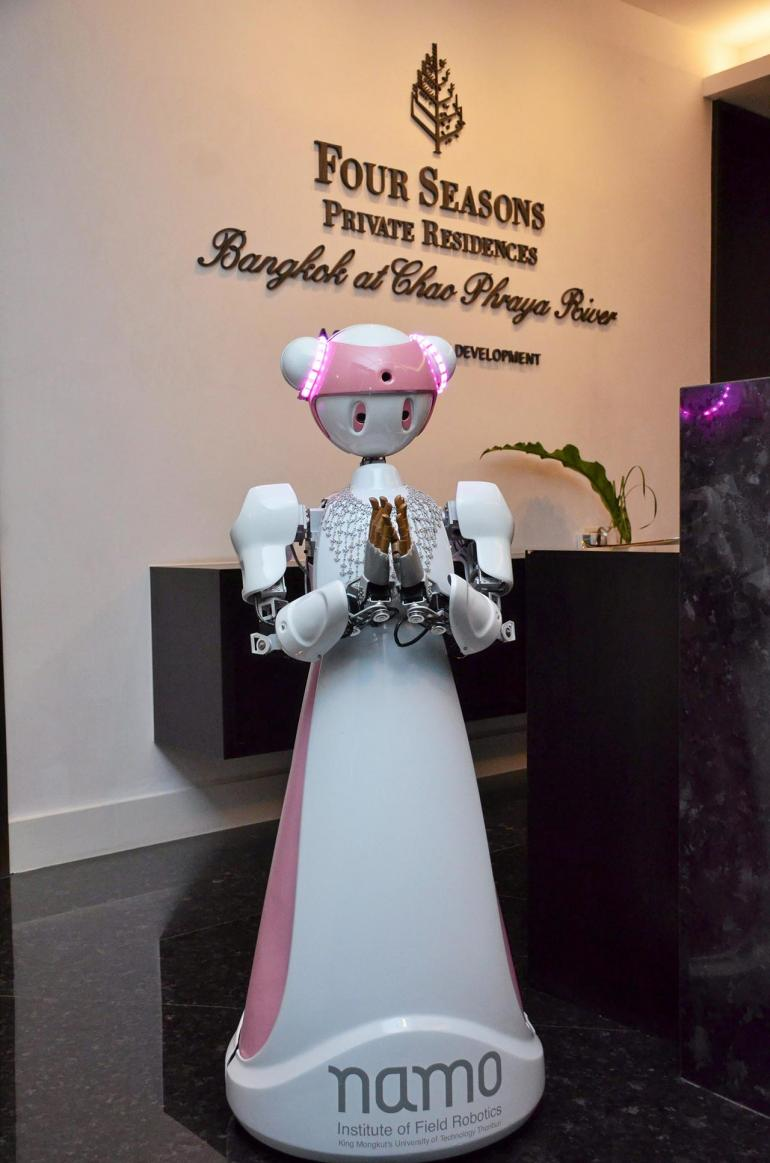
\includegraphics[width=\textwidth]{chapter2/images/namo.jpg}
        \caption{หุ่นยนต์ประชาสัมพันธ์นะโม}
        \label{fig:namo}
    \end{subfigure}
    \hfill
    \begin{subfigure}[b]{0.3\textwidth}
        \centering
        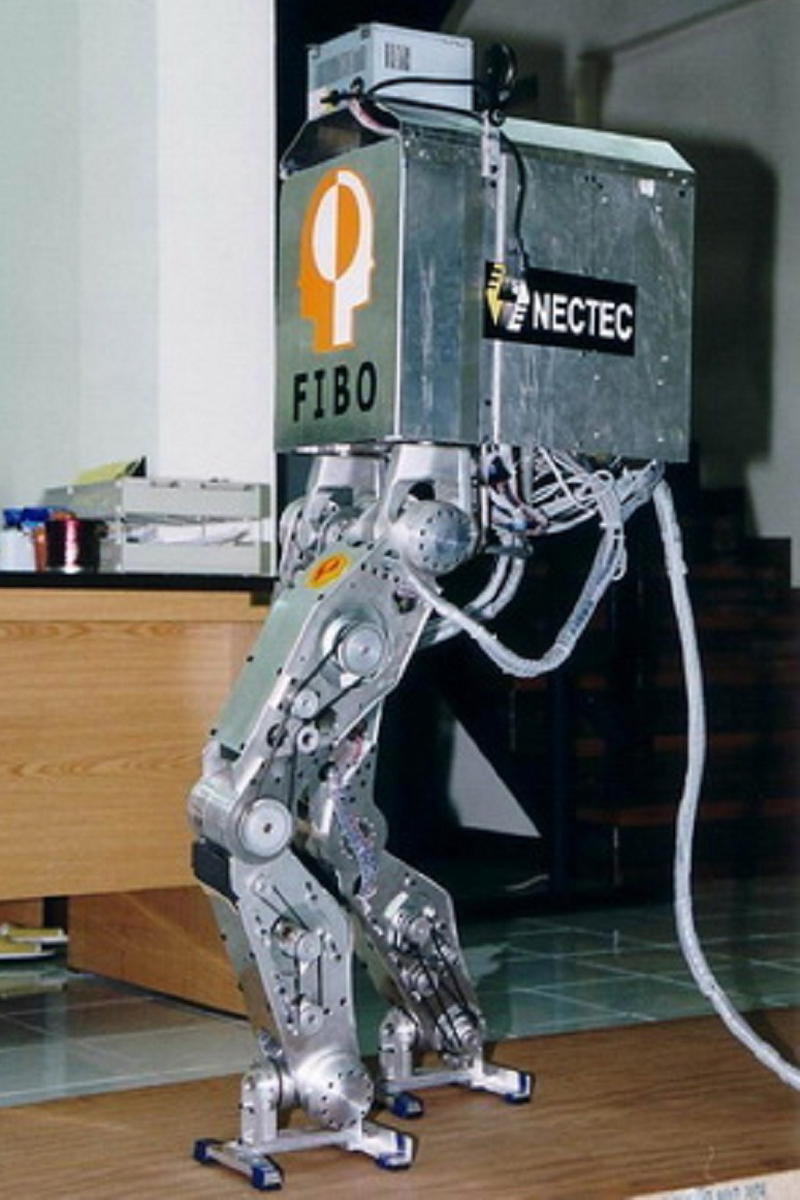
\includegraphics[width=\textwidth]{chapter2/images/ส้มจุก.jpg}
        \caption{หุ่นยนต์เดินสองขาส้มจุก}
        \label{fig:ส้มจุก}
    \end{subfigure}
    \hfill
    \begin{subfigure}[b]{0.3\textwidth}
        \centering
        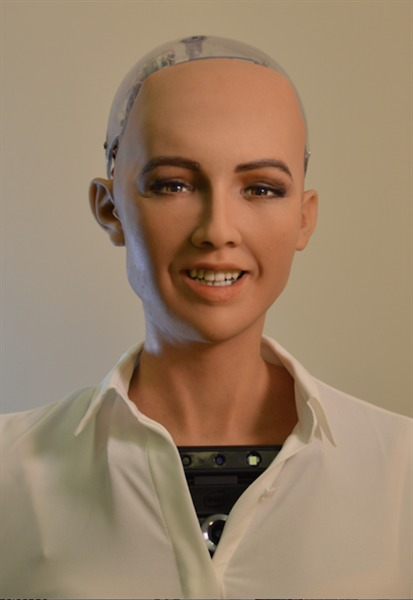
\includegraphics[width=\textwidth]{chapter2/images/โซเฟีย.jpg}
        \caption{หุ่นยนต์แอนดรอยด์โซเฟีย}
        \label{fig:โซเฟีย}
    \end{subfigure}
    \caption{แสดงความแตกต่างของหุ่นยนต์ฮิวมานอยด์แต่ละประเภท}
    \label{fig:diff_humanoid}
\end{figure}

งานวิจัยทางด้านหุ่นยนต์ฮิวมานอยด์จากอดีตจนถึงปัจจุบันส่วนใหญ่จะเป็นการพัฒนาความสามารถของการเดินของหุ่นยนต์
เช่น เริ่มต้นจากแรกสุดจะเป็นการพัฒนาให้หุ่นยนต์สามารถเดินหน้าได้ ต่อมาก็เพิ่มความสามารถให้หุ่นยนต์สามารถเดินบนพื้นเอียง พื้นขรุขระ
เดินเลี้ยวซ้ายขวา เดินขึ้นลงบันได ฯลฯ เป็นต้น นอกจากนี้ยังมีการพัฒนาปรับปรุงสมดุลของการเดินแบบสองขาอีกด้วย สมดุลของการเดินสามารถแบ่งได้สองแบบหลัก
คือ การเดินแบบสมดุลสถิต และการเดินแบบสมดุลพลวัต งานในยุคแรกนั้นจะพัฒนาให้เดินได้แบบสมดุลสถิต ต่อมาเป็นสมดุลกึ่งพลวัต
และเป็นสมดุลพลวัต การพัฒนาตัวควบคุมการเดินของหุ่นยนต์ จำเป็นที่จะต้องใช้ความรู้ทางด้านกลศาสตร์ค่อนข้างมาก มีการใช้สมการที่มีความซับซ้อน

Zheng และคณะ (1988) พัฒนาหุ่นยนต์สองขาที่สามารถเดินบนพื้นราบได้ ให้สามารถเดินต่อเนื่องไปบนพื้นเอียงได้ด้วย
พื้นเอียงที่ใช้มีลักษณะเป็นพื้นเอียงขึ้น หุ่นยนต์ที่ใช้ในงานนี้มีข้อต่อสะโพก (hip), ข้อเท้า (ankle) และลำตัว (torso) มีเซนเซอร์วัดแรงกด (force sensor)
ติดตั้งอยู่ที่ปลายเท้าและส้นเท้าแต่ละข้างเพื่อใช้วัดตำแหน่งของน้ำหนักโดยรวม (center of gravity) ของหุ่นยนต์ การเดินของงานวิจัยจะพิจารณาเฉพาะการเดินในแนวหน้าหลัง
โดยมีหลักการคือ การเดินบนพื้นเอียงโดยที่หุ่นยนต์ยังเดินในท่าทางเหมือนกับตอนที่เดินบนพื้นราบจะทำให้น้ำหนักโดยรวมของหุ่นยนต์เลื่อนไปข้างหลัง
ดังนั้นการที่หุ่นยนต์ขยับลำตัวไปด้านหน้าจำทำให้น้ำหนักโดยรวมของหุ่นยนต์กลับมาอยู่ตรงกลางของพื้นที่รับน้ำหนักเหมือนเดิม
ซึ่งจะทำให้หุ่นยนต์มีความสมดุลได้ ดั้งนั้นข้อมูลที่ได้จากหน่วยวัดแรงกดที่เท้าจะถูกนำมาคำนวณตลอดการเดินเพื่อใช้ในการปรับเปลี่ยนมุมการขยับของลำตัว
การเดินบนพื้นราบเป็นแบบสมดุลสถิตและการเดินบนพื้นเอียงก็ยังคงเป็นแบบสมดุลสถิตเช่นกัน

Inaba และคณะ (1995) สร้างหุ่นยนต์เลียนแบบลิง (ape-like biped) ประกอบด้วยสองมือและสองขา มีการเดินแบบสมดุลสถิต
งานวิจัยนี้มีความคิดว่านอกจากการทำให้หุ่นยนต์สองขาเดินได้โดยไม่ล้มแล้ว ควรจะทำหุ่นยนต์ที่สามารถลุกขึ้นเองได้หลังจากที่ล้มแล้วด้วย
ดังนั้นในงานนี้ หุ่นยนต์ถูกพัฒนาให้สามารถเดิน เมื่อล้มแล้วก็สามารถพลิกตัวและลุกขึ้นมาเดินให้ได้

Kun และ Miller (1996) ได้นำโครงข่ายประสาทเทียม มาประยุกต์ใช้ในการปรับเปลี่ยนท่าทางการเดินโดยอัตโนมัติของหุ่นยนต์สองขา
การที่หุ่นยนต์สามารถปรับเปลี่ยนท่าทางได้โดยอัตโนมัตินี้มีประโยชน์ทำให้หุ่นยนต์เดินได้บนพื้นผิวหลากหลายลักษณะมากขึ้น
ในงานนี้พิจารณาท้ังสมดุลในแนวหน้าหลัง (sigittal plane) และแนวซ้ายขวา (frontal plane) และการเดินของหุุ่นยนต์เป็นแบบสมดุลพลวัต
หลักการทำงานประกอบด้วยตัวสร้างท่าทางการเดินหนึ่งตัว และตัวปรับท่าทางการเดินทั้งแนวหน้าหลังและซ้ายขวาอีกหนึ่งตัว
โดยค่าการปรับเปลี่ยนนั้นจะได้มาจาก แรงกดที่เท้า ความยาวการก้าวเท้า ความสูงของการยกเท้า เป็นต้น นอกจากนี้
ในปีถัดมาทั้งสิงได้ใช้หลักการที่ใช้ในงานนี้ไปใช้กับการเดินของหุ่นยนต์อีกตัว (Kun and Miller, 1997)

Hirai และคณะ (1998) พัฒนาหุ่นยนต์ฮิวมานอยด์ ซึ่งตัวหุ่นยนต์มีความคล้ายมนุษย์มาก สามารถเดินได้อย่างราบลื่นคล้านมนุษย์มากที่สุด
เช่น สามารถเดินได้ในพื้นผิวชนิดต่างๆ เดินได้บนพื้นเอียงขึ้นเอียงลง เดินขึ้นลงบันได้ได้ เดินเข็นรถได้ เป็นต้น การเดินในทุกสถานการณ์เป็นการเดินแบบสมดุลพลวัต
หุ่นยนต์สามารถเดินได้ด้วยความเร็วสูงสุด 4.7 กิโลเมตรต่อชั่วโมง หุ่นยนต์ประกอบไปด้วย แขนข้างละ 9 องศาอิสระ ขาข้างละ 6 องศาอิสระ
ที่บริเวณหัวมีกล้องติดตั้งอยู่ 4 ตัว นอกจากนี้ยังมีอุปกรณ์ที่ใช้ในการรักษาสมดุลอื่นๆ อีกได้แก่ IMU ที่ติดตั้งบริเวณลำตัว และ Force sensor ที่ติดที่เท้าทั้งสองข้าง

\clearpage
ส่วนประกอบของหุ่นยนต์ฮิวมานอยด์สามารถจำแนกออกเป็นส่วนหลักๆได้สามส่วนคือ 
ส่วนการรับรู้ ส่วนการประมวลผล และส่วนการขับเคลื่อน

\subsubsection*{การรับรู้ของหุ่นยนต์ฮิวมานอยด์}
การรับรู้ของหุ่นยนต์ฮิวมานอยด์นั้นมีความยากมากกว่าหุ่นยนต์ชนิดอื่นๆเพราะหุ่นยนต์จะมีการเคลื่อนที่ และการเคลื่อนที่นั้นทำให้เซนเซอร์โดนรบกวนได้
ยกตัวอย่างเช่น ภาพที่ได้จากกล้องนั้นอาจจะเบลอได้ถ้าความเร็วของชัตเตอร์ช้าเกินไป หรือว่าภาพเปลี่ยนขณะที่กำลังกดชัตเตอร์
ข้อมูลตำแหน่งของตัวเองก็มีความแน่นอนที่น้อยกว่าหุ่นยนต์เคลื่อนที่ด้วยล้อ เพราะเซนเซอร์ที่วัดตำแหน่งเทียบกับเฟรมโลกไม่มีความเสถียร
หุ่นยนต์ที่เคลื่อนที่ด้วยล้อปกติถ้าติดกล้อง ตัวกล้องจะมีความสูงจากพื้นคงที่ แต่หุ่นยนต์ฮิวมานอยด์ไม่ใช่ โดยหุ่นยนต์ฮิวมานอยด์นั้นจะต้องมีการคำนวณ
forward kinematics จากเท้าที่สัมผัสกับพื้นมายังกล้องเพื่อหาตำแหน่งและการหมุนของกล้อง ส่วนการวัดตำแหน่งของตัวหุ่นยนต์นั้น
โดยทั่วไปแล้วจะใช้เซนเซอร์ inertia measurement unit (IMU) และเซนเซอร์ Encoders สำหรับหาตำแหน่งของข้อต่อต่างๆ
ปกติจะติดเซนเซอร์ IMU ไว้ที่ลำตัวของหุ่นยนต์ใกล้ๆกับ center of mass ของหุ่นยนต์ ส่วน Encoder นั้นจะติดไว้ที่ข้อต่อของหุ่นยนต์

\subsubsection*{การประมวลผลของหุ่นยนต์ฮิวมานอยด์}
ในปัจจุบันนี้หุ่นยนต์ฮิวมานอยด์มีความสามารถในการคำนวณที่สูงมากเมื่อเทียบกับเมื่อก่อน บอร์ดที่เราสามารถเห็นได้โดยทั่วไปเช่น
Raspberry Pi, Odroid, Intel NUCs ซึ่งตัวบอร์ดมีขนาดเล็กจึงทำให้เข้าไปอยู่ในตัวของหุ่นยนต์ได้ แถมบอร์ดพวกนี้ยังมี GPUs
และ CPU หลายคอร์อีกด้วย บางครั้งก็มีคนที่เอาพวกบอร์ดพวกนี้มาทำงานร่วมกันหลายๆตัว ประมวลผลแบบ pararell เพื่อที่จะเพิ่มประสิทธิภาพในการประมวลผล
โดยเชื่อมต่อระหว่างกันผ่าน Ethernet network 

\subsubsection*{การขับเคลื่อนของหุ่นยนต์ฮิวมานอยด์}
หุ่นยนต์ฮิวมานอยด์ส่วนใหญ่จะมีข้อต่ออยู่หลายๆจุด แต่ละข้อต่อจะมีตัวขับเคลื่อน ตัวขับเคลื่อนมีอยู่หลักๆสองแบบคือ
แบบกล้ามเนื่อของมนุษย์ และแบบมอเตอร์ที่ติดตรงที่ข้อต่อเลย ที่นิยมใช้คือแบบมอเตอร์ที่ติดที่ข้อต่อเลย เพราะทำให้ตัวของหุ่นยนต์มีขนาดเล็ก
ใช้พื้นที่น้อย การใช้เส้นเอ็นดึงนั้นจะการจะทำให้ข้อต่อไปยังตำแหน่งที่ต้องการได้ยากกว่า ตัวขับเคลื่อนนั้นต้องการแรงมากน้อยขึ้นอยู่กับ
น้ำหนักของตัวหุ่นยนต์ เพื่อที่จะทำให้หุ่นยนต์นั้นยังยืนได้

\clearpage
\subsection{ทฤษฏีที่เกี่ยวข้องกับมนุษย์}
\subsubsection{การวิเคราะห์การเดินของมนุษย์}
การเคลื่อนที่ของหุ่นยนต์ฮิวมานอยด์นั้นจะเลียนแบบมาจากการเดินของมนุษย์
ดั้งนั้นการวิเคราะห์ลักษณะการเดินของมนุษย์ จะเป็นการศึกษาเพื่อทำความเข้าใจถึงธรรมชาติการเดิน
ก่อนนำไปทำการออกแบบกลไกทางกลและระบบควบคุมของหุ่นยนต์ฮิวมานอยด์
การก้าวเดินของมนุษย์โดยปกติแล้ว จะมีลักษณะเป็นวัฏจักร วนซ้ำไปเรื่อยๆ ในทิศทางที่ต้องการจนกว่าจะทำการหยุดเดิน
การทรงตัวในระหว่างการยืนหรือการเดินนั้น เป็นไปตามสัญชาติญาณซึ่งเกิดจากการรักษาความสมดุลของระดับน้ำในหู\footnote{text}
ส่งสัญญาณผ่านเส้นประสาทไปยังกล้ามเนื้อส่วนต่างๆ ที่ทำหน้าที่ให้เกิดการเคลื่อนที่

การเคลื่อนที่ของมนุษย์ในการเดินไปข้างหน้าสามารถแบ่งออกเป็นช่วงต่างๆดังนี้
\begin{figure}[htbp]
    \centering
    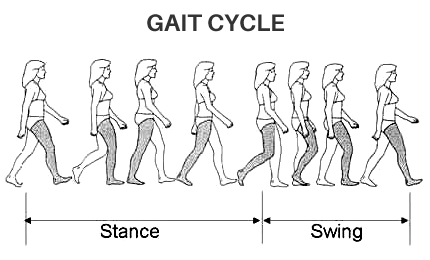
\includegraphics[width=0.55\textwidth]{chapter2/images/gaitcycle.png}
    \caption{วัฏจักรการเดินของมนุษย์}
    \label{fig:human_gait_cycle}
\end{figure}
\begin{enumerate}[label=\arabic*., leftmargin=1.5cm]
    \item ช่วงเริ่มการวางเท้าเพื่อเข้าสู่ช่วงเริ่มต้นเหวี่ยงเท้า เป็นช่วงที่เท้าเกิดการกระแทกลงบนพื้นหลังจากทำการเหวี่ยงมาจากด้านหลัง
    โดยธรรมชาติมนุษย์จะทำการวางส้นเท้าลงเพื่อลดแรงกระแทกที่เกิดขึ้นในช่วงนี้
    ดังนั้นทางกายภาพในส่วนของส้นเท้ามนุษย์จึงมีลักษณะอ่อนนุ่ม
    \item ช่วงเริ่มต้นเหวี่ยงเท้าเพื่อเข้าสู่ช่วงเหวี่ยงเท้า หลังจากทำการวางส้นเท้าลงกับพื้นแล้ว ข้อเข้าจะปรับมุมเพื่อให้ฝ่าเท้าแนบพื้นสนิท
    ขณะเดียวกันขาอีกข้างจะยกสูงขึ้นเพื่อถ่ายเทน้ำหนักไปยังเท้าที่เพิ่งวางลง
	\item ช่วงเหวี่ยงเท้า เป็นช่วงที่ขาหนึ่งยกลอยอยู่ในอากาศและขาที่วางแนบกับพื้นจะรองรับน้ำหนักทั้งหมดของร่างกาย
	\item ช่วงเตรียมการวางเท้า เป็นช่วงที่ขาข้างที่ลอยอยู่เหวี่ยงไปข้างหน้าเพื่อเตรียมเข้าสู่ช่วงรองรับ 
    ในขณะเดียวกันขาที่รับน้ำหนักอยู่จะทำการผลักตัวเพื่อเริ่มทำการถ่ายเทน้ำหนักไปข้างหน้า
\end{enumerate}

\subsubsection{การวิเคราะห์องศาอิสระของมนุษย์}
การที่มนุษย์เราสามารถเคลื่อนที่ได้นั้น เป็นผลเนื่องมาจากการเคลื่อนที่ของข้อต่อต่าง ๆ ที่อยู่
บนขา ซึ่งประกอบไปด้วย ข้อต่อส่วนสะโพก ข้อต่อส่วนหัวเข่า และข้อต่อส่วนข้อเท้า แรงบิดที่เกิด
ขึ้นของแต่ละข้อต่อมีความสัมพันธ์ต่อกัน ส่งผลให้เกิดเสถียรภาพในการเดินของมนุษย์ เมื่อวิเคราะห์
ลักษณะโครงสร้างในแต่ละส่วน พบว่าข้อต่อส่วนสะโพกมีลักษณะเป็นทรงกลม ทำให้ข้อต่อส่วน
สะโพกสามารถหมุนได้ 3 องศาอิสระ ส่วนหัวเข่าของมนุษย์ มีจุดต่อของข้อที่มีลักษณะเป็นทรงกลม
สองลูกประกอบเข้าด้วยกันทำให้การเคลื่อนที่ถูกบังคับให้สามารถเคลื่อนที่ได้เพียง 1 องศาอิสระ ใน
ส่วนของข้อเท้ามีลักษณะการเคลื่อนที่เหมือนสะโพกคือสามารถเคลื่อนที่ได้ 3 องศาอิสระ

จากทั้งหมดที่ได้ทำการวิเคราะห์มาข้างต้นพบว่าในขาหนึ่งข้างของมนุษย์ประกอบด้วย 7 องศาอิสระ
ซึ่งส่งผลให้การเคลื่อนที่ของมนุษย์มีความคล่องแคล่วสูง แต่ในทางออกแบบกลไกการเดินและการควบคุม
ของหุ่นยนต์สองขาถือว่ามีจำนวนองศาอิสระเกินความจำเป็นในการเคลื่อนที่บนปริภูมิ(space) และยากต่อ
การควบคุม(under actuated) ดังนั้นการกำหนดจำนวนองศาอิสระเพื่อให้หุ่นยนต์เดินได้เสมือนมนุษย์จึง
มีผลในการออกแบบกลไกทางกลและการควบคุมของหุ่นยนต์สองขา 

\subsubsection{กายวิภาคศาสตร์}


\subsection{ทฤษฏีที่เกี่ยวข้องกับหุ่นยนต์ฮิวมานอยด์}
\subsubsection{ส่วนประกอบของหุ่นยนต์ฮิวมานอยด์}
\begin{figure}[ht]
	\centering
	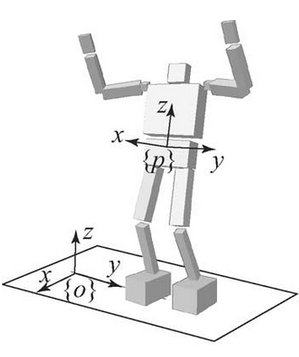
\includegraphics[width=0.4\textwidth]{chapter2/images/robot_component.png}
	\caption{ส่วนประกอบของหุ่นยนต์ฮิวมานอยด์}
	\label{fig:robot_component}
\end{figure}
หุ่นยนต์ฮิวมานอยด์ประกอบด้วยก้านต่อหลายๆก้านที่นำมาต่อกัน ลักษณะโครงสร้างนั้นจะเป็นแบบโซ่เปิด (Open kinematic chain)
และแต่ละก้านต่อจะเชื่อมต่อกันด้วยข้อต่อแบบหมุน เราสามารถแบ่งโครงสร้างของหุ่นยนต์ฮิวมานอยด์ออกเป็นส่วนหลักๆเป็น 2 ส่วน ส่วนแรกคือ
ส่วนก้านต่อของลำตัวหุ่นยนต์ (Torso) ซึ่งเราสามารถที่จะรวมไปถึงส่วนแขนกับหัวด้วย
และในส่วนที่สองคือ ส่วนก้านต่อของขาหุ่นยนต์ (Legs) ซึ่งเป็นส่วนขาของหุ่นยนต์ทั้งสองข้างที่สามารถนำไปที่สัมผัสกับพื้นได้
ทั้งสองก้านต่อนี้ถูกเชื่อมต่อกันด้วยส่วนของสะโพก (Hip) ที่อยู่ระหว่างส่วนลำตัวกับส่วนของขาหุ่นยนต์ ดังรูปที่ \ref{fig:robot_component}

\subsubsection{วัฏจักรการเดินของหุ่นยนต์ฮิวมานอยด์}
วัฏจักรการเดินของหุ่นยนต์ คือ การที่หุ่นยนต์จะต้องมีการถ่ายน้ำหนักไปมาระหว่างเท้าซ้ายและเท้าขวา
มีบางช่วงที่น้ำหนักตกลงบนเท้าข้างใดข้างหนึ่งหรือทั้งสองข้างพร้อมกัน สามารถแบ่งออกเป็นช่วงได้สองช่วง คือช่วงการยืนด้วยขาข้างเดียว
และช่วงการยืนด้วยขาทั้งสองข้าง
\begin{figure}[!ht]
	\centering
	\begin{subfigure}[b]{0.22\textwidth}
		\centering
		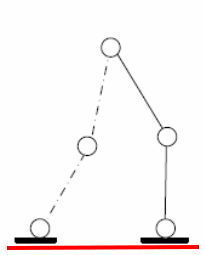
\includegraphics[width=\textwidth]{chapter2/images/doublesupport.png}
		\caption{ยืนด้วยขาสองข้าง}
		\label{fig:robot_walk_1}
	\end{subfigure}
	\hfill
	\begin{subfigure}[b]{0.45\textwidth}
		\centering
		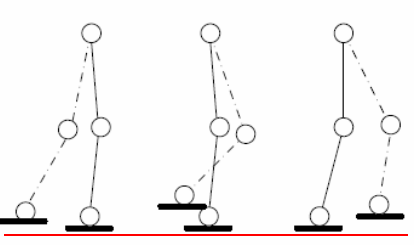
\includegraphics[width=\textwidth]{chapter2/images/singlesupport.png}
		\caption{ยืนด้วยขาข้างเดียว}
		\label{fig:robot_walk_2}
	\end{subfigure}
	\hfill
	\begin{subfigure}[b]{0.22\textwidth}
		\centering
		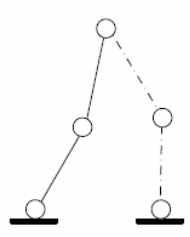
\includegraphics[width=\textwidth]{chapter2/images/doublesupport2.png}
		\caption{ยืนด้วยขาสองข้าง}
		\label{fig:robot_walk_3}
	\end{subfigure}
	\caption{วัฐจักรการเดินของหุ่นยนต์ฮิวมานอยด์}
	\label{fig:robot_walk_phase}
\end{figure}

\clearpage
\paragraph*{1) การยืนด้วยขาข้างเดียว :}
เป็นช่วงที่มีเท้าของหุ่นยนต์สัมผัสพื้นเพียงข้างเดียว ส่วนเท้าอีกข้างของหุ่นยนต์จะถูกยกลอยจากพื้น
โดยที่ไม่มีส่วนใดๆของขาข้างนั้นสัมผัสกับพื้นเลย ช่วงนี้จะเกิดขึ้นเมื่อมีการแกว่งเท้าจากข้างหลังไปข้างหน้า
ดังรูปที่ \ref{fig:robot_walk_2}

\paragraph*{2) การยืนด้วยขาสองข้าง :}
เป็นช่วงที่เท้าทั้งสองข้างของหุ่นยนต์สัมผัสกับพื้น ช่วงนี้จะเกิดตั้งแต่หุ่นยนต์วางเท้าขณะที่ส้นเท้าแตะกับพื้น
ไปจนถึง ปลายเท้าของขาอีกข้างหลุดออกจากพื้น

การเดินได้โดยไม่ล้มนั้น ตัวหุ่นยนต์จะต้องรักษาสมดุลของการเดินให้ได้ตลอดช่วงเวลาของการเดิน
ซึ่งสมดุลของการเดินแบบสองขาสามารถแบ่งตามลักษณะการเดินและการถ่ายน้ำหนักได้เป็น 2 รูปแบบหลัก คือ 
การเดินแบบสมดุลสถิต (static balance walking) และ การเดินแบบสมดุลพลวัต (dynamic balance walking)

\subsubsection{การสร้างและการควบคุมการเดินแบบสมดุลสถิต}
การเดินของหุ่นยนต์ในลักษณะนี้ จุดศูนย์กลางมวล (CoM) ของตัวหุ่นยนต์จะไม่มีการเคลื่อนไหวออกนอกบริเวณฐานรับน้ำหนัก (Supporting Area)
ตลอดช่วงเวลาการเดิน ไม่ว่าจะเป็นช่วงเวลาที่รับน้ำหนักด้วยเท้าข้างเดียวหรือทั้งสองข้างก็ตาม หมายความว่า โครงสร้างของหุ่นยนต์จะไม่ล้มแน่นอน
เนื่องจากการสร้างรูปแบบการเดินด้วยวิธีนี้จะควบคุมให้ตำแหน่งของจุดศูนย์กลางมวล อยู่ภายในพื้นที่ฐานรับน้ำหนักของหุ่นยนต์ตลอดเวลา
\ref{Legged robots walk the walk,https://blog.csiro.au/legged-robots-walk-walk/}

\begin{figure}[ht]
	\centering
	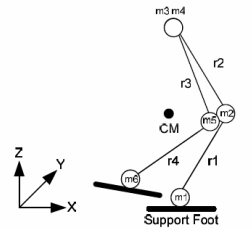
\includegraphics[width=0.4\textwidth]{chapter2/images/cominsupportpolygon.png}
	\caption{การควบคุมตำแหน่งของจุดรวมมวลให้อยู่ในพื้นที่ฐาน}
	\label{fig:robot_com_support}
\end{figure}

ข้อดีของการสร้างและควบคุมการเดินของหุ่นยนต์ด้วยวิธีนี้คือ สามารถสร้างรูปแบบการเดินได้โดยที่มีความซับซ้อนไม่มากนัก
สามารถสั่งให้หุ่นยนต์หยุดค้างในท่าทางใดๆก็ได้ตลอดเวลาโดยหุ่นยนต์ไม่ล้ม หุ่นยนต์ที่มีฝ่าเท้าใหญ่จะทำให้ง่ายต่อการก้าวเดินมากขึ้น
นอกจากการควบคุมการก้าวขาแล้วอาจเพิ่มการควบคุมส่วนลำตัวเพิ่มเติม เพื่อเป็นการเพิ่มเสถียรภาพในการเดินและการถ่ายเทน้ำหนัก
โดยที่อาจจะมีการเพิ่มเซนเซอร์วัดแรงที่ฝ่าเท้าเพื่อตรวจสอบการกระจายแรงกดที่ฝ่าเท้า เพื่อตรวจสอบว่าตำแหน่งของจุดรวมน้ำหนักอยู่บนพื้นที่ฝ่าเท้าหรือไม่
หรือเพื่อตรวจสอบเสถียรภาพของการเดินเพื่อแก้ไขท่าทางการเดินไม่ให้เกิดการล้ม

ข้อเสียของการควบคุมการเดินด้วยวิธีนี้คือ หุ่นยนต์จะใช้เวลาในการก้าวเดินมาก ใช้พลังงานในการเดินมากกว่าการเดินแบบสมดุลพลวัต
และท่าทางที่ได้จะมีความแตกต่างจากท่าทางการเดินของมนุษย์

\subsubsection{การสร้างและการควบคุมการเดินแบบสมดุลพลวัต}
การสร้างรูปแบบการเดินและควบคุมการเดินในลักษณะนี้ท่าทางการเดินของหุ่นยนต์นั้นจะคล้ายกับการเดินของมนุษย์มากกว่าแบบสถิต
เนื่องจากมีหลักการในการสร้างท่าทางที่เหมือนกับการเดินของมนุษย์ซึ่งมีขั้นตอนดังนี้คือ เอียงตัวให้ล้มไปในทิศทางที่ต้องการเดิน
เมื่อเริ่มเกิดการล้มขึ้นหุ่นยนต์จะเปลี่ยนตำแหน่งการวางเท้าไปยังตำแหน่งใหม่ เพื่อปรับให้โครงสร้างเข้าสู่สภาวะสมดุลอีกครั้ง

โดยธรรมชาติแล้วมนุษย์มีการถ่ายน้ำหนักในขณะที่เคลื่อนที่หรือยืนอยู่กับที่เพื่อรักษาสมดุลของท่าทางนั้นไว้
แต่หากการถ่ายโอนน้ำหนักนั้นเกิดสภาวะไม่สมดุล ร่างกายจะปรับสภาพโดยการเคลื่อนตำแหน่งของเท้าซึ่งเป็นพื้นที่ฐานออกจากเดิมไปยังตำแหน่งใหม่
เพื่อรักษาสมดุลไว้ หลักการดังกล่าวถูกนำมาใช้กับการควบคุมการเดินของหุ่นยนต์ฮิวมานอยด์ ในขณะที่หุ่นยนต์กำลังเคลื่อนไหว
ผลจากแรงเฉื่อยของการเคลื่อนที่และผลจากแรงดึงดูดของโลกมีผลต่อการเพิ่มและลดความเร่งให้การเดินของหุ่นยนต์
แรงเหล่านี้เรียกว่าแรงเฉื่อยรวมของการเคลื่อนที่ และเมื่อเท้าหุ่นยนต์สัมผัสกับพื้นจะได้รับผลกระทบของแรงนี้ เรียกว่า
แรงปฏิกิริยาจากพื้น

การตัดกันระหว่างแรงปฏิกิริยาจากพื้นและแนวแรงเฉื่อยรวม ตำแหน่งนั้นหากทำให้โมเมนต์เท่ากับศูนย์
เรียกจุดตัดนี้ว่าจุดโมเมนต์ศูนย์ ($ZMP_{robot}$) และจุดที่แรงปฏิกิริยาลงสู่พื้นว่า จุดปฏิกิริยาพื้นฐาน 
ท่าทางการเดินของหุ่นยนต์จะถูกกำหนดและถูกส่งให้กับชุดควบคุมข้อต่อจุดต่างๆของหุ่นยนต์ โดยให้สอดคล้องกับแรงเฉื่อยรวมที่เกิดขึ้นจากการคำนวณ
เรียกว่าแรงเฉื่อยรวมเป้าหมาย และจุดโมเมนต์ศูนย์ที่ได้จากการคำนวณเรียกว่าจุดโมเมนต์ศูนย์เป้าหมาย ($ZMP_{target}$)
เมื่อหุ่นยนต์เกิดสมดุลในขณะที่ทำการเดินได้อย่างสมบูรณ์ แนวแกนของแรงเฉื่อยรวมเป้าหมายและแรงปฏิกิริยาที่พื้นจะเป็นตำแหน่งเดียวกัน
แต่ในขณะที่หุ่นยนต์เดินผ่านพื้นผิวที่มีความขรุขระหรือไม่เรียบตำแหน่งสองจุดดังกล่าง จะไม่ใช่ตำแหน่งเดียวกันทำให้หุ่นยนต์เกิดการล้มได้
แรงที่ทำให้เกิดการล้มนี้เกิดจากตำแหน่งของจุดโมเมนต์ศูนย์และตำแหน่งแรงปฏิกิริยารวมที่พื้นไม่ตรงกัน ซึ่งเป็นสาเหตุหลักที่ทำให้เกิดความไม่สมดุลขึ้น
และเมื่อหุ่นยนต์เสียสมดุลระบบที่จะสามารถป้องกันการล้มและทำให้หุ่นยนต์เดินต่อไปได้อย่างต่อเนื่องคือ ระบบควบคุมแรงปฏิกิริยา
ระบบควบคุมจุดโมเมนต์ศูนย์ และระบบควบคุมการวางเท้า\ref{Achieving Stable walking,http://world.honda.com/ASIMO/history/technology2.html}

\begin{figure}[!ht]
	\centering
	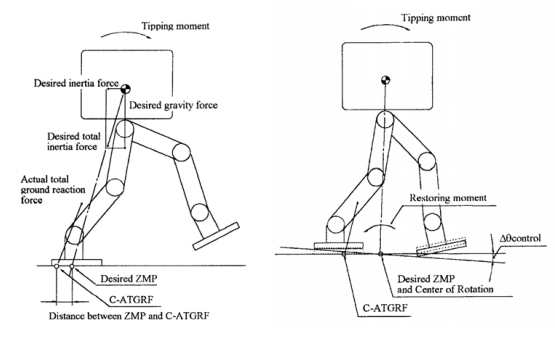
\includegraphics[width=0.7\textwidth]{chapter2/images/zmpdynamicwalking.png}
	\caption{การควบคุมตำแหน่งของจุดโมเมนต์ศูนย์ให้ตรงกับแรงปฏิกิริยารวม}
	\label{fig:robot_zmp_support}
\end{figure}

อย่างไรก็ตาม การสร้างท่าทางการเดินในลักษณะนี้ต้องใช้สมการในการคำนวณที่ซับซ้อนมาก
เนื่องจากต้องหาความสัมพันธ์ระหว่างองค์ประกอบหลายส่วน เช่น น้ำหนักของโครงสร้างในแต่ละส่วน 
แรงบิดที่แต่ละข้อต่อ และโมเมนต์โดยรวมของระบบ นอกจากนี้ยังต้องใช้อุปกรณ์การตรวจวัดต่างๆ เช่น เซนเซอร์วัดแรง
เซนเซอร์วัดมุม เซนเซอร์วัดแรงบิด ติดตั้งตามจุดต่างๆของโครงสร้างเพื่อวัดค่าออกมา ก่อนที่จะทำการคำนวณตำแหน่ง
และสร้างท่าทางการเดินของหุ่นยนต์ฮิวมานอยด์ ท่าทางการเดินที่ได้จากการควบคุมด้วยวิธีนี้ จะมีความคล้ายคลึงกับท่าทางการเดินของมนุษย์มาก

\subsubsection{จุดศูนย์กลางมวลของหุ่นยนต์}
หากต้องการให้หุ่นยนต์สามารถที่จะทรงตัวอยู่ได้โดยไม่ล้มนั้น จึงต้องรู้ตำแหน่งจุดศูนย์กลางมวลของหุ่นยนต์ตลอดเวลา
และต้องให้จุดศูนย์กลางมวลฉายตกในบริเวณฐานรับน้ำหนักของหุ่นยนต์โดยหาจากพื้นที่ที่ฝ่าเท้าสัมผัสกับพื้น
วิธีการนี้เป็นวิธีการทางสถิตศาสตร์

\clearpage
\section{งานวิจัยที่เกี่ยวข้อง}
\subsection{ตัวอย่างหุ่นยนต์ฮิวมานอยด์}
\subsection*{Poppy Humanoid}
\begin{figure}[htbp]
    \centering
    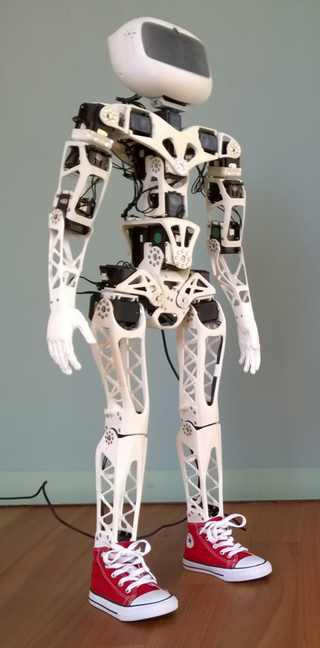
\includegraphics[width=0.3\textwidth]{chapter2/images/PoppyHumanoid1.png}
    \caption{หุ่นยนต์ฮิวมานอยด์ป๊อปปี้}
    \label{fig:poppy_humanoid}
\end{figure}
หุ่นยนต์ฮิวมานอยด์ป๊อปปี้ ถูกสร้างขึ้นมาเพื่อใช้ในงานศิลปะ การวิจัยและการศึกษาโดยเฉพาะ 
หุ่นยนต์ป๊อปปี้ประกอบด้วยส่วนของฮาร์ทแวร์และซอฟแวร์ที่เปิดเป็นโอเพนซอร์ซให้ผู้ที่สนใจสามารถเข้ามาศึกษาได้
โปรแกรมของหุ่นยนต์ใช้โมดูลที่มีชื่อว่า Pypot ที่เป็นส่วนเสริมของภาษา Python ในการพัฒนาซอฟแวร์
ทุกคนสามารถเข้าถึงข้อมูลเชิงเทคนิคของหุ่นยนต์ฮิวมานอยด์ป๊อปปี้ได้ เช่น ส่วนรายละเอียดการทำงาน
คลิปวีดีโอสอนการประกอบ การใช้ระบบจำลอง และการพัฒนาต่างๆผ่านทางเว็บไซต์ http://www.poppy-project.org 
หุ่นยนต์ป๊อปปี้มีส่วนของโครงสร้างที่ผลิตมาจากพลาสติด PLA และ ABS โดยใช้เทคนิคการขึ้นรูปด้วยเครื่องพิมพ์สามมิติ
ตัวขับเคลื่อนข้อต่อต่างๆใช้เป็น Dynamixel Digital Servo และควบคุมคำสั่งของตัวขับเคลื่อนด้วย 
คอมพิวเตอร์ขนาดเล็ก Odroid UX4 ใช้ระบบปฎิบัติการ Ubuntu 14.04 
ตัวของหุ่นยนต์มีความสูง 83 เซนติเมตร น้ำหนัก 3.5 กิโลกรัม 
ใช้เซนเซอร์วัดมุมเอียงเป็น IMU ที่มีองศาอิสระเท่ากับ 9 องศาอิสระ ในการควบคุมเสถียรภาพในการเดินของตัวเอง
มีองศาอิสระหรือจำนวนตัวขับเคลื่อนทั้งหมด 25 องศา ประกอบไปด้วย ขาข้างละ 6 องศาอิสระ แขนข้างละ 4 องศาอิสระ 
ลำตัว 3 องศาอิสระ และ หัว 2 องสาอิสระ

\clearpage
\subsection*{iCub Humanoid}
\begin{figure}[htbp]
    \centering
    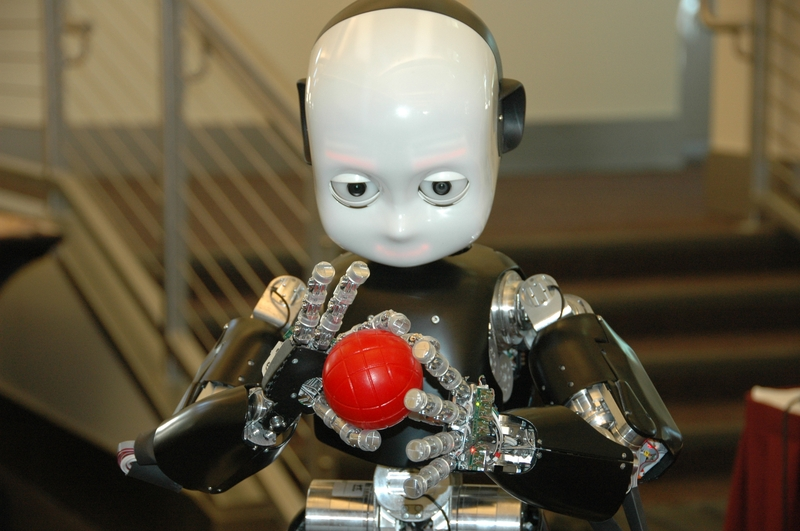
\includegraphics[width=0.6\textwidth]{chapter2/images/icub-1.jpg}
    \caption{หุ่นยนต์ฮิวมานอยด์ไอคัพ}
    \label{fig:icub_humanoid}
\end{figure}
หุ่นยนต์ฮิวมานอยด์ไอคัพ ถูกออกแบบโดยมหาวิทยาลัยหลายแห่งในยุโรปรวมกลุ่มกันขึ้นมาในชื่อ RobotCub
และถูกสร้างขึ้นโดย Istituto Italiano di Tecnologia (IIT) ตัวหุ่นยนต์ไอคัพนั้นมีความสูงอยู่ที่ 1 เมตร
น้ำหนักโดยรวมทั้งหมดประมาณ 22 กิโลกรัม วัสดุที่ใช้ในการสร้างแตกต่างกันไปในแต่ละส่วนของร่างกายโดยจะใช้
aluminum alloy AI6082 สำหรับส่วนที่ต้องรับภาระความเครียดน้อย ใช้ aluminum alloy 7075(Ergal) สำหรับส่วนที่ต้องรับภาระความเครียดปานกลางถึงสูง
และใช้ Stainless Steel 17-4PH ในส่วนของเพลาข้อต่อต่างๆเพื่อให้มีความแข็งแรงสูง ตัวหุ่นยนต์ถูกออกแบบให้มีลักษณะเหมือนเด็กอายุ 3-4 ขวบ
ควบคุมโดยใช้บอร์ดไมโครคอนโทรเลอร์เป็นรุ่น PC104 Controller ภาษาที่ใช้ในการพัฒนาใช้เป็นภาษา C++ ในการเขียนโปรแรม
การติดต่อสื่อสารกับตัวขับเคลื่อนหรือมอเตอร์ตามข้อต่อต่างๆ และเซนเซอร์ ผ่านทางโปรโตคอล CAN Bus เพื่อทำให้ใช้สายน้อยลง
ใช้เส้นเอ็นในการส่งถ่ายแรงขับเคลื่อนไปยังส่วนของข้อต่อส่วนมือและไหล่ นิ้วของหุ่นยนต์ถูกร้อยด้วย สายเคเบิลเคลือบ Teflon อยู่ภายใน
และคลายตัวกลับสู่สภาวะสมดุลได้ด้วยแรงของสปริง เซนเซอร์วัดมุมของข้อต่อแต่ละตัวใช้การออกแบบให้มี Hall-effect ติดอยู่
ช่วยในการอ่านค่าของตำแหน่งและความเร็วที่เกิดขึ้นที่ข้อต่อนั้น หุ่นยนต์ไอคัพมีองศาอิสระรวมกันทั้งหมด 53 องศาอิสระ
ประกอบไปด้วย แขนข้างละ 7 องศาอิสระ มือข้างละ 9 องศาอิสระ หัว 6 องศาอิสระ ลำตัว 3 องศาอิสระ และขาข้างละ 6 องศาอิสระ
ในส่วนของหัวจะประกอบไปด้วย กล้องสองตัวเพื่อทำสเตอริโอวิชั่น ไมโครโฟนสำหรับรับเสียงจากสภาพแวดล้อมภายนอก
และไฟแสดงอารมณ์บริเวณปากและคิ้ว หุ่นยนต์นี้ไม่ได้ถูกออกแบบให้มีการทำงานเป็นแบบอัตโนมัติ ซึ่งก็คือตัวหุ่นยนต์นั้นไม่มีแบตเตอรี่ภายในตัว
แต่ใช้แหล่งพลังงานจากภายนอกโดยการส่งเข้าไปผ่านสายเคเบิล และเชื่อมต่อกับอินเทอร์เน็ตผ่านสายแลน (LAN)

\clearpage
\subsection*{Darwin-OP Humanoid}
\begin{figure}[htbp]
    \centering
    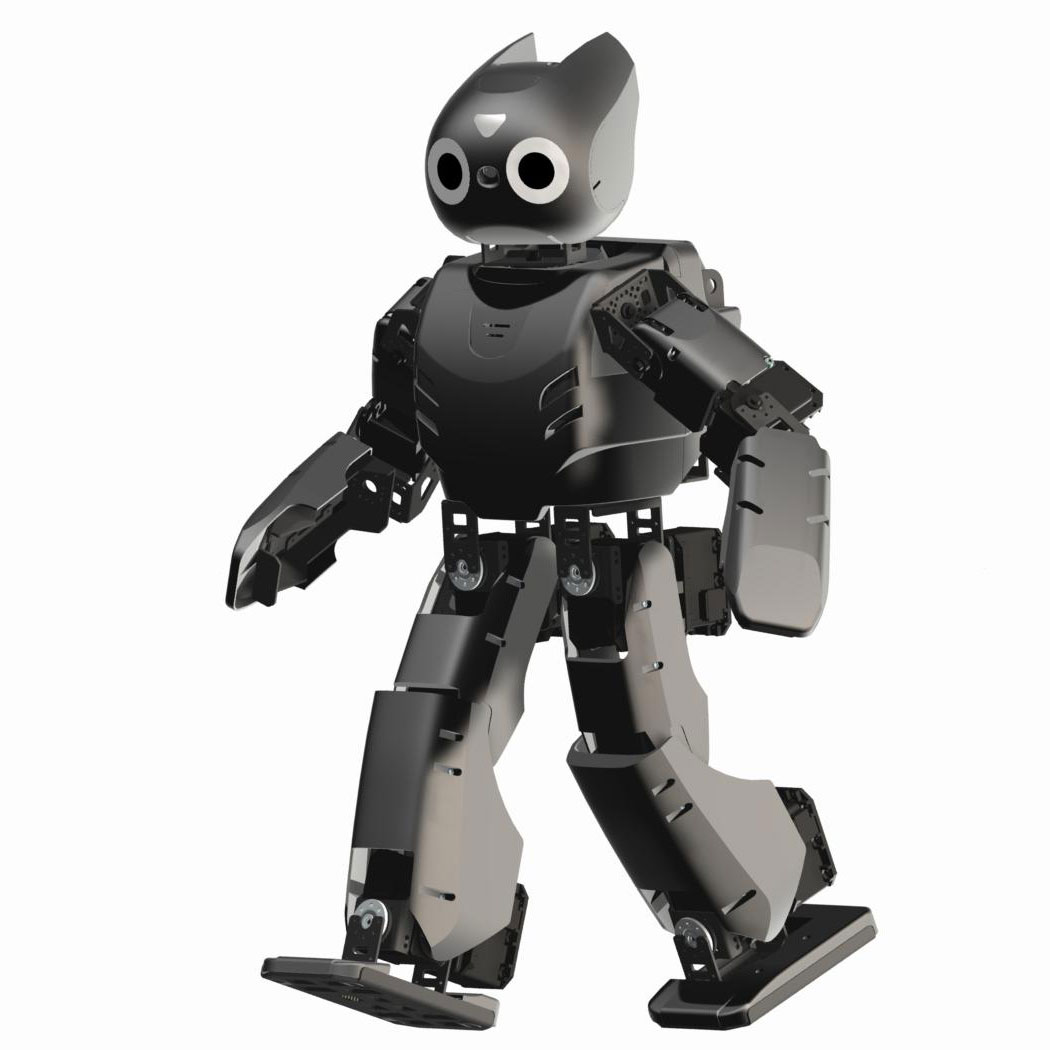
\includegraphics[width=0.55\textwidth]{chapter2/images/Darwin_OP_6.jpg}
    \caption{หุ่นยนต์ฮิวมานอยด์ดาร์วิน}
    \label{fig:darwin_humanoid}
\end{figure}
หุ่นยนต์ฮิวมานอยด์ดาร์วิน (Darwin-OP) เป็นชื่อที่ย่อมาจากคำว่า Dynamic Anthropomorphic Robot
with Intelligence–Open Platform
เป็น OpenSource Platform ที่ถูกออกแบบและพัฒนาโดย Korean robot manufacturer Robotis
โดยมีความร่วมมือกับ Virginia polytechnic institude and state university, Purdue university และ University of Pennsylvania
หุ่นยนต์ฮิวมานอยด์ดาร์วินมีความสามารถในการรับภาระโหลดได้สูง เนื่องจากมีการพัฒนามอเตอร์เป็นของตัวเอง อีกทั้งยังมีความสามารถในการเคลื่อนที่แบบ
พลวัต (Dynamic) หุ่นยนต์ดาร์วิน มีองศาอิสระทั้งหมด 20 องศาอิสระ ซึ่งประกอบไปด้วย ขาข้างละ 6 องศาอิสระ แขนข้างละ 3 องศาอิสระ และหัว 2 องศาอิสระ
ขับเคลื่อนข้อต่อต่างๆด้วยเซอร์โวมอเตอร์ Dynamixel MX-28T ที่มีการเชื่อมต่อแบบ RS485 ในการประหยัดสายที่ใช้ในการสั่งการ มอเตอร์แต่ละตัวมีเซนเซอร์วัดตำแหน่ง 
และความเร็วอยู่ภายใน ตัวหุ่นยนต์มีความสูงทั้งหมด 45 เซนติเมตร มีน้ำหนักโดยประมาณ 2.9 กิโลกรัม
ระบบภายในใช้คอมพิวเตอร์ขนาดเล็กเป็น 1.6 GHz Intel Atom Z530 (32 bit) ใช้คอนโทรเลอร์ ARM CortexM3 STM32F103RE 72 MHz 
และมีเซนเซอร์วัดมุมเอียงเป็น 3-axis gyro, 3-axis accelerometer เพื่อช่วยในการควบคุมเสถียรภาพในการเดิน

\clearpage
\subsection*{Nao Humanoid}
\begin{figure}[htbp]
    \centering
    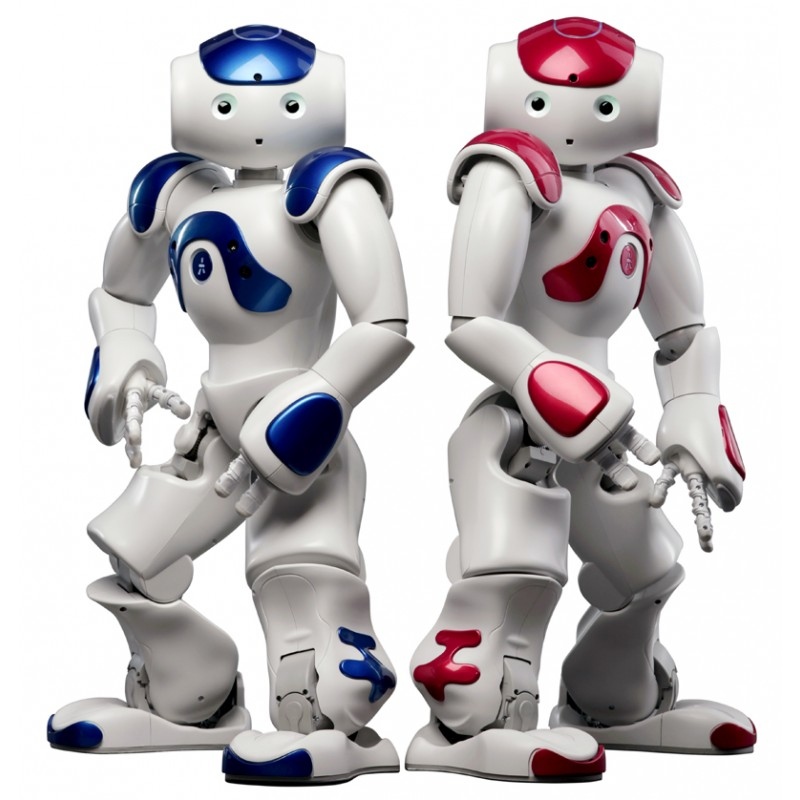
\includegraphics[width=0.55\textwidth]{chapter2/images/nao.jpg}
    \caption{หุ่นยนต์ฮิวมานอยด์นาโอะ}
    \label{fig:nao_humanoid}
\end{figure}
หุ่นยนต์ฮิวมานอยด์นาโอะ เป็นหุ่นยนต์ฮิวมานอยด์ขนาดกลาง ถูกผลิตมาจากประเทศฝรั่งเศษ พัฒนาโดยบริษัท Aldebaran Robotics เมื่อปี 2004 และในปี 2007
หุ่นยนต์ฮิวมานอยด์นาโอะได้นำไปแทนที่หุ่นยนต์สุนัขของ Sony ชื่อ Aibo ขณะถูกใช้ในรายการแข่งขัน RoboCup Standard Platform League (SPL) หุ่นยนต์นาโอะได้ถูกนำไปใช้ใน Robocup 2008 และ 2009 
หุ่นยนต์นาโอะถูกพัฒนาออกมาหลายรุ่นมีองศาอิสระตั้งแต่ 14 องศาอิสระ 21 องศาอิสระ และ 25 องศาอิสระ สำหรับเพื่องานวิจัยนั้นมีถึง 25 องศาอิสระ
โดยเพิ่มเติมมือสองข้างเอาเข้าไปเพื่อให้สามารถหยิบจับสิ่งของได้ ภายในหุ่นยนต์ถูกควบคุมด้วยระบบปฎิบัติการ NAO 2.0 (Linux-based) ตัวหุ่นยนต์มีความสูง 58 เซนติเมตร 
น้ำหนัก 4.3 กิโลกรัม ส่วนเซนเซอร์การรับรู้ต่างๆจะประกอบไปด้วย เซนเซอร์วัดมุมเอียง 3-axis gyro, 3-axis accelerometer, Ultrasound captors, ไมโครโฟน 4 ตัว ลำโพง 2 ตัว กล้อง 2 ตัว เพื่อใช้ประโยชน์ในการทำงานวิจัยต่างๆ
ตอนนี้ความสามารถของหุ่นยนต์นาโอะที่ทำได้คือ สามารถเทน้ำส้มได้ เดินขึ้นลงบันไดและทางลาดชันได้ ระหว่างการเดินนั้นสามารถวางแผนการวางเท้าได้อย่างรวดเร็ว
อีกทั้งยังสามารถที่จะเดินหลบหลีกสิ่งกีดขวางได้ด้วย

\clearpage
\subsection*{Wabot}
\begin{figure}[htbp]
    \centering
    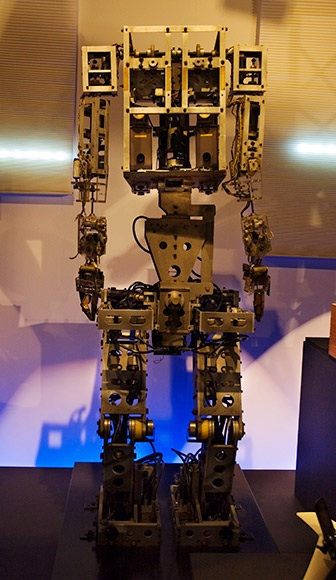
\includegraphics[width=0.45\textwidth]{chapter2/images/wabot.jpg}
    \caption{หุ่นยนต์ฮิวมานอยด์วาบอท}
    \label{fig:wabot_humanoid}
\end{figure}
หุ่นยนต์ฮิวมานอยด์มีการพัฒนาในช่วงแรกเริ่มมาตั้งแต่ปี 1973 หุ่นยนต์ฮิวมานอยด์ ตัวแรกชื่อ Wabot-1 เริ่มสร้างโดยมหาวิทยาลัย Waseda ที่ประเทศญี่ปุ่น ตัวของหุ่นยนต์มีความสูง 180 เซนติเมตร
น้ำหนัก 210 กิโลกรัม โดยหุ่นยนต์สามารถติดต่อสื่อสารกับมนุษย์ได้ด้วยภาษาญี่ปุ่น สามารถวัดระยะและทิศทางได้โดยใช้การรับรู้ผ่านทางตาและหูเทียม หุ่นยนต์ Wabot-1 นั้นสามารถเดินได้ด้วยขาของตนเองที่มีสองข้าง
สามารถหยิบและเคลื่อนย้ายวัตถุด้วยมือ ต่อมาในปี 1984 มหาวิทยาลัย Waseda ได้พัฒนาหุ่นยนต์ฮิวมานอยด์ที่ชื่อ Wabot-2 โดยหุ่นยนต์สามารถสื่อสารกับมนุษย์ได้ สามารถอ่านโน๊ตเพลงและเล่นดนตรีโดยใช้ electronic organ แบบง่ายๆได้
และในปี 1985 บริษัท Hitachi ได้สร้างหุ่นยนต์ WHL-11 ที่มีสองขาเหมือนมนุษย์ ซึ่งสามารถเดินแบบสมดุลสถิต (Static Walking) บนพื้นราบได้ด้วยความเร็ว 13 วินาทีต่อหนึ่งก้าว และสามารถเลี้ยวได้ซ้ายและขวาได้


\clearpage
\subsection{งานวิจัยการออกแบบระบบหุ่นยนต์ฮิวมานอยด์}


